\hypertarget{build-a-conversational-ai-system-with-jaseci}{%
\section{Build a Conversational AI System with
Jaseci}\label{build-a-conversational-ai-system-with-jaseci}}

In this tutorial, you are going to learn how to build a state-of-the-art
conversational AI system with Jaseci and the Jac language. You will
learn the basics of Jaseci, training state-of-the-art AI models, and
everything in between, in order to create an end-to-end fully-functional
conversational AI system.

Excited? Hell yeah! Let's jump in.

\hypertarget{preparation}{%
\subsection{Preparation}\label{preparation}}

To install jaseci, run this in your development environment:

\begin{lstlisting}
pip install jaseci
\end{lstlisting}

To test the installation is successful, run:

\begin{lstlisting}
jsctl --help
\end{lstlisting}

\passthrough{\lstinline!jsctl!} stands for the Jaseci Command Line
Interface. If the command above displays the help menu for
\passthrough{\lstinline!jsctl!}, then you have successfully installed
jaseci.

\begin{quote}
\textbf{Note}

Take a look and get familiarized with these commands while you are at
it. \passthrough{\lstinline!jsctl!} will be frequently used throughout
this journey.
\end{quote}

\hypertarget{background}{%
\subsection{Background}\label{background}}

A few essential concepts to get familiar with.

\hypertarget{graph-nodes-edges}{%
\subsubsection{Graph, nodes, edges}\label{graph-nodes-edges}}

Refer to relevant sections of the Jaseci Bible.

\hypertarget{walker}{%
\subsubsection{Walker}\label{walker}}

Refer to relevant sections of the Jaseci Bible.

\hypertarget{automated-faq-answering-chatbot}{%
\section{Automated FAQ answering
chatbot}\label{automated-faq-answering-chatbot}}

Our conversational AI system will consist of multiple components. To
start, we are going to build a chatbot that can answer FAQ questions
without any custom training, using zeroshot NLP models. At the end of
this section, you will have a chatbot that, when given a question,
searches in its knowledge base for the most relevant answer and returns
that answer.

The use case here is a Tesla FAQ chatbot. We will be using the list of
FAQs from https://www.tesla.com/en\_SG/support/faq.

\begin{quote}
\textbf{Note}

This architecture works for any FAQ topics and use cases. Feel free to
pick another product/website/company's FAQ if you'd like!
\end{quote}

\hypertarget{define-the-nodes}{%
\subsection{Define the Nodes}\label{define-the-nodes}}

We have 3 different types of nodes:

\begin{itemize}
\tightlist
\item
  \passthrough{\lstinline!root!}: This is the root node of the graph. It
  is a built-in node type and each graph has one root node only.
\item
  \passthrough{\lstinline!faq\_root!}: This is the entry point of the
  FAQ handler. We will make the decision on the most relevant answer at
  this node.
\item
  \passthrough{\lstinline!faq\_state!}: This node represents a FAQ
  entry. It contains a candidate answer from the knowledge base.
\end{itemize}

Now let's define the custom node types.

\begin{lstlisting}
node faq_root;
node faq_state {
    has question;
    has answer;
}
\end{lstlisting}

The \passthrough{\lstinline!has!} keyword defines a node's variables. In
this case, each \passthrough{\lstinline!faq\_state!} has a
\passthrough{\lstinline!question!} and \passthrough{\lstinline!answer!}.

\begin{quote}
\textbf{Warning}

The \passthrough{\lstinline!root!} node does not need explicit
definition. It is a built-in node type. Avoid using
\passthrough{\lstinline!root!} as a custom node type.
\end{quote}

\hypertarget{build-the-graph}{%
\subsection{Build the Graph}\label{build-the-graph}}

For this FAQ chatbot, we will build a graph as illustrated here:

\begin{figure}
\centering
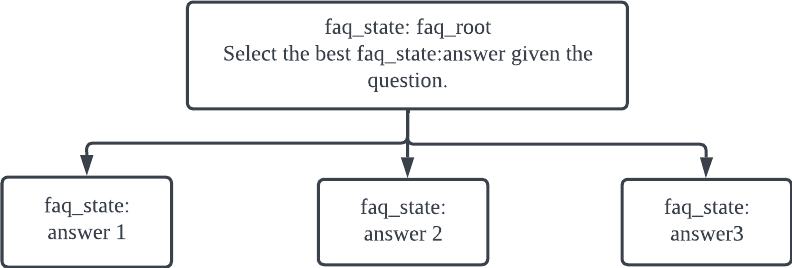
\includegraphics{images/faq_1.png}
\caption{Architecture of FAQ Bot}
\end{figure}

The idea here is that we will decide which FAQ entry is the most
relevant to the incoming question at the
\passthrough{\lstinline!faq\_root!} node and then we will traverse to
that node to fetch the corresponding answer.

To define this graph architecture:

\begin{lstlisting}
// Static graph definition
graph faq {
    has anchor faq_root;
    spawn {
        // Spawning the nodes
        faq_root = spawn node::faq_root;
        faq_answer_1 = spawn node::faq_state(
            question="How do I configure my order?",
            answer="To configure your order, log into your Tesla account."
        );
        faq_answer_2 = spawn node::faq_state(
            question="How do I order a tesla",
            answer="Visit our design studio to place your order."
        );
        faq_answer_3 = spawn node::faq_state(
            question="Can I request a test drive",
            answer="Yes. You must be a minimum of 25 years of age."
        );

        // Connecting the nodes together
        faq_root --> faq_answer_1;
        faq_root --> faq_answer_2;
        faq_root --> faq_answer_3;
    }
}
\end{lstlisting}

Let's break down this piece of code.

We observe two uses of the \passthrough{\lstinline!spawn!} keyword. To
spawn a node of a specific type, use the \passthrough{\lstinline!spawn!}
keyword for:

\begin{lstlisting}
faq_answer_1 = spawn node::faq_state(
    question="How do I configure my order?",
    answer="To configure your order, log into your Tesla account.",
);
\end{lstlisting}

In the above example, we just spawned a
\passthrough{\lstinline!faq\_state!} node called
\passthrough{\lstinline!faq\_answer\_1!} and initialized its
\passthrough{\lstinline!question!} and \passthrough{\lstinline!answer!}
variables.

\begin{quote}
\textbf{Note}

The \passthrough{\lstinline!spawn!} keyword can be used in this style to
spawn many different jaseci objects, such as nodes, graphs and walkers.
\end{quote}

The second usage of \passthrough{\lstinline!spawn!} is with the graph:

\begin{lstlisting}
graph faq {
    has anchor faq_root;
    spawn {
       ...
    }
}
\end{lstlisting}

In this context, the \passthrough{\lstinline!spawn!} designates a code
block with programmatic functionality to spawn a subgraph for which the
root node of that spawned graph will be the
\passthrough{\lstinline!has anchor faq\_root!}.

In this block:

\begin{itemize}
\tightlist
\item
  We spawn 4 nodes, one of the type \passthrough{\lstinline!faq\_root!}
  and three of the type \passthrough{\lstinline!faq\_state!}.
\item
  We connect each of the faq answer states to the faq root with
  \passthrough{\lstinline!faq\_root --> faq\_answer\_*!}.
\item
  We set the \passthrough{\lstinline!faq\_root!} as the anchor node of
  the graph. As we will later see, spawning a graph will return its
  anchor node.
\end{itemize}

\begin{quote}
\textbf{Warning}

An anchor node is required for every graph block. It must be assigned
inside the spawn block of the graph definition.
\end{quote}

\hypertarget{initialize-the-graph}{%
\subsection{Initialize the Graph}\label{initialize-the-graph}}

Similar to nodes, in order to create the graph, we will use the
\passthrough{\lstinline!spawn!} keyword.

\begin{lstlisting}
walker init {
    root {
        spawn here ++> graph::faq;
    }
}
\end{lstlisting}

This is the first walker we have introduced, so let's break it down.

\begin{itemize}
\tightlist
\item
  The walker is called \passthrough{\lstinline!init!}.
\item
  It contains logic specifically for the \passthrough{\lstinline!root!}
  node, meaning that the code inside the
  \passthrough{\lstinline!root \{\}!} block will run \textbf{only} on
  the \passthrough{\lstinline!root!} node. This syntax applies for any
  node types, as you will see very soon. Every Jac program starts with a
  single root node, but as you will later learn, a walker can be
  executed on any node, though the root is used by default if none is
  specified.
\item
  \passthrough{\lstinline!spawn here ++> graph::faq!} creates an
  instance of the \passthrough{\lstinline!faq!} graph and connects its
  anchor node to \passthrough{\lstinline!here!}, which is the node the
  walker is currently on.
\end{itemize}

\begin{quote}
\textbf{Note}

\passthrough{\lstinline!init!} can be viewed as similar to
\passthrough{\lstinline!main!} in Python. It is the default walker to
run when no specific walkers are specified for a
\passthrough{\lstinline!jac run!} command.

\passthrough{\lstinline!here!} is a very powerful keyword. It always
evaluates to the specific node the walker is currently on. You will be
using \passthrough{\lstinline!here!} a lot throughout this tutorial.
\end{quote}

\hypertarget{run-the-init-walker}{%
\subsection{\texorpdfstring{Run the \texttt{init}
Walker}{Run the init Walker}}\label{run-the-init-walker}}

Now, let's run the init walker to initialize the graph. First put all of
the above code snippet into a single jac file and name it
\passthrough{\lstinline!main.jac!}, including

\begin{itemize}
\tightlist
\item
  nodes definition
\item
  graph definition
\item
  init walker
\end{itemize}

Run \passthrough{\lstinline!jsctl!} to get into the jaseci shell
environment:

\begin{lstlisting}[language=bash]
jsctl
\end{lstlisting}

Inside the \passthrough{\lstinline!jsctl!} shell,

\begin{lstlisting}[language=bash]
jaseci > jac dot main.jac
\end{lstlisting}

This command runs the \passthrough{\lstinline!init!} walker of the
\passthrough{\lstinline!main.jac!} program and prints the state of its
graph in DOT format after the walker has finished.
\href{https://graphviz.org/doc/info/lang.html}{The DOT language} is a
popular graph description language widely used for representing complex
graphs.

The output should look something like this

\begin{figure}
\centering
\includegraphics{images/dot_1.png}
\caption{Dot output for Faq graph}
\end{figure}

\begin{lstlisting}
strict digraph root {
    "n0" [ id="0955c04e4ff945b4b836748ef2bbd98a", label="n0:root"  ]
    "n1" [ id="c1240d79110941c1bc2feb18581951bd", label="n1:faq_root"  ]
    "n2" [ id="55333be285c246db88181ac34d16cd20", label="n2:faq_state"  ]
    "n3" [ id="d4fa8f2c46ca463f9237ef818e086a29", label="n3:faq_state"  ]
    "n4" [ id="f7b1c8ae82af4063ad53646adc5544e9", label="n4:faq_state"  ]
    "n0" -> "n1" [ id="a718fd6c938149269d3ade2af2eb023c", label="e0" ]
    "n1" -> "n2" [ id="3757cb15851249b4b6083d7cb3c34f8e", label="e1" ]
    "n1" -> "n4" [ id="626ce784a8f5423cae5d5d5ca857fc5c", label="e2" ]
    "n1" -> "n3" [ id="a609e7b54bde4a6a9c9711afdb123241", label="e3" ]
}
\end{lstlisting}

\begin{quote}
\textbf{Note}

We are not going to cover the DOT syntax. There are many resources
online if you are interested, e.g.,
https://graphviz.org/doc/info/lang.html
\end{quote}

\begin{quote}
\textbf{Note}

There are tools available to render a graph in DOT format. For example,
https://dreampuf.github.io/GraphvizOnline has a WSIWYG editor to render
dot graph in real time.
\end{quote}

Congratulations! You have just created your first functional jac
program!

\hypertarget{ask-the-question}{%
\subsection{Ask the Question}\label{ask-the-question}}

Alright, we have initialized the graph. Now it's time to create the code
for the question-answering. We will start with a simple string matching
for the answer selection algorithm. For this, we will create a new
walker called \passthrough{\lstinline!ask!}.

\begin{lstlisting}
walker ask {
    has question;
    root {
        question = std.input("AMA > ");
        take --> node::faq_root;
    }
    faq_root {
        take --> node::faq_state(question==question);
    }
    faq_state {:
        std.out(here.answer);
    }
}
\end{lstlisting}

This walker is more complex than the \passthrough{\lstinline!init!} one
and introduces a few new concepts so let's break it down!

\begin{itemize}
\tightlist
\item
  Similar to nodes, walkers can also contain
  \passthrough{\lstinline!has!} variables. They define variables of the
  walker. They can also be passed as parameters when calling the walker.
\item
  \passthrough{\lstinline!std.input!} and
  \passthrough{\lstinline!std.out!} read and write to the command line
  respectively.
\item
  This walker has logic for three types of node:
  \passthrough{\lstinline!root!}, \passthrough{\lstinline!faq\_root!}
  and \passthrough{\lstinline!faq\_state!}.

  \begin{itemize}
  \tightlist
  \item
    \passthrough{\lstinline!root!}: It simply traverses to the
    \passthrough{\lstinline!faq\_root!} node.
  \item
    \passthrough{\lstinline!faq\_root!}: This is where the answer
    selection algorithm is. We will find the most relevant
    \passthrough{\lstinline!faq\_state!} and then traverse to that node
    via a \passthrough{\lstinline!take!} statement. In this code
    snippet, we are using a very simple (and limited) string matching
    approach to try to match the predefined FAQ question with the user
    question.
  \item
    \passthrough{\lstinline!faq\_state!}: Print the answer to the
    terminal.
  \end{itemize}
\end{itemize}

Before we run this walker, we are going to update the
\passthrough{\lstinline!init!} walker to speed up our development
process

\begin{lstlisting}
walker init {
    root {
        spawn here ++> graph::faq;
        spawn here walker::ask;
    }
}
\end{lstlisting}

This serves as a shorthand so that we can initialize the graph and ask a
question in one command.

\begin{quote}
\textbf{Note}

This demonstrates how one walker can spawn another walker using the
\passthrough{\lstinline!spawn!} keyword.
\end{quote}

Time to run the walker!

\begin{lstlisting}[language=bash]
jaseci > jac run main.jac
\end{lstlisting}

\passthrough{\lstinline!jac run!} functions very similarly to
\passthrough{\lstinline!jac dot!}, with the only difference being that
it doesn't return the graph in DOT format. Try giving it one of the
three questions we have predefined and it should respond with the
corresponding answer.

\hypertarget{introducing-universal-sentence-encoder}{%
\subsection{Introducing Universal Sentence
Encoder}\label{introducing-universal-sentence-encoder}}

Now, obviously, what we have now is not very ``AI'' and we need to fix
that. We are going to use the Universal Sentence Encoder QA model as the
answer selection algorithm. Universal Sentence Encoder is a language
encoder model that is pre-trained on a large corpus of natural language
data and has been shown to be effective in many NLP tasks. In our
application, we are using it for zero-shot question-answering, i.e.~no
custom training required.

Jaseci has a set of built-in libraries or packages that are called
Jaseci actions. These actions cover a wide-range of state-of-the-art AI
models across many different NLP tasks. These actions are packaged in a
Python module called \passthrough{\lstinline!jaseci\_ai\_kit!}.

To install \passthrough{\lstinline!jaseci\_ai\_kit!}:

\begin{lstlisting}[language=bash]
pip install jaseci_ai_kit
\end{lstlisting}

Now we load the action we need into our jaseci environment

\begin{lstlisting}[language=bash]
jaseci > actions load module jaseci_ai_kit.use_qa
\end{lstlisting}

Let's update our walker logic to use the USE QA model:

\begin{lstlisting}
walker ask {
    can use.qa_classify;
    has question;
    root {
        question = std.input(">");
        take --> node::faq_root;
    }
    faq_root {
        answers = -->.answer;
        best_answer = use.qa_classify(
            text = question,
            classes = answers
        );
        take --> node::faq_state(answer==best_answer["match"]);
    }
    faq_state {
        std.out(here.answer);
    }
}
\end{lstlisting}

Even though there are only 5 lines of new code, there are many
interesting aspects, so let's break it down!

\begin{itemize}
\tightlist
\item
  \passthrough{\lstinline!-->.answer!} collects the
  \passthrough{\lstinline!answer!} variable of all of the nodes that are
  connected to
  \passthrough{\lstinline!here!}/\passthrough{\lstinline!faq\_root!}
  with a \passthrough{\lstinline!-->!} connection.
\item
  \passthrough{\lstinline!use.qa\_classify!} is one of the action
  supported by the USE QA action set. It takes in a question and a list
  of candidate answers and return the most relevant one.
\end{itemize}

Now let's run this new updated walker and you can now ask questions that
are relevant to the answers beyond just the predefined ones.

\hypertarget{scale-it-out}{%
\subsection{Scale it Out}\label{scale-it-out}}

So far we have created a FAQ bot that is capable of providing answer in
three topics. To make this useful beyond just a prototype, we are now
going to expand its database of answers. Instead of manually spawning
and connecting a node for each FAQ entry, we are going to write a walker
that automatically expands our graph:

\begin{lstlisting}
walker ingest_faq {
    has kb_file;
    root: take --> node::faq_root;
    faq_root {
        kb = file.load_json(kb_file);
        for faq in kb {
            answer = faq["answer"];
            spawn here ++> node::faq_state(answer=answer);
        }
    }
}
\end{lstlisting}

An example knowledge base file look like this

\begin{lstlisting}
[
  {
    "question": "I have a Model 3 reservation, how do I configure my order?",
    "answer": "To configure your order, log into your Tesla Account and select manage on your existing reservation to configure your Tesla. Your original USD deposit has now been converted to SGD."
  },
  {
    "question": "How do I order a Tesla?",
    "answer": "Visit our Design Studio to explore our latest options and place your order. The purchase price and estimated delivery date will change based on your configuration."
  },
  {
    "question": "Can I request a Test Drive?",
    "answer": "Yes, you can request for a test drive. Please note that drivers must be a minimum of 25 years of age and not exceeding 65 years of age, hold a full driving license with over 2 years of driving experience. Insurance conditions relating to your specific status must be reviewed and accepted prior to the test drive."
  }
]
\end{lstlisting}

Save the above json in a file named
\passthrough{\lstinline!tesla\_faq.json!} and make sure it is in the
same location as \passthrough{\lstinline!main.jac!}. Let's now update
the \passthrough{\lstinline!init!} walker. Because we are going to use
the \passthrough{\lstinline!ingest\_faq!} walker to generate the graph,
we won't need the static graph definition.

\begin{lstlisting}
walker init {
    root {
        spawn here ++> node::faq_root;
        spawn here walker::ingest_faq(kb_file="tesla_faq.json");
        spawn here walker::ask;
    }
}
\end{lstlisting}

What we are doing here is

\begin{itemize}
\tightlist
\item
  Spawning a \passthrough{\lstinline!faq\_root!} node
\item
  Running the \passthrough{\lstinline!ingest\_faq!} walker to create the
  neccessary \passthrough{\lstinline!faq\_state!} nodes based on the
  question-answer entries in the
  \passthrough{\lstinline!tesla\_faq.json!} file.
\item
  Launching the \passthrough{\lstinline!ask!} walker
\end{itemize}

Let's run the program one more time and test it out!

\begin{lstlisting}[language=bash]
jaseci > jac run main.jac
\end{lstlisting}

\begin{quote}
\textbf{Note}

Try more varied questions. Now we have a longer answer with more rich
information, it has a higher coverage of information that will be able
to answer more questions.
\end{quote}

\begin{quote}
\textbf{Note}

If you are feeling adventurous, try downloading the complete list of
entires on the Tesla FAQ page and use it to create a production-level
FAQ bot. See if you can push the model to its limit!
\end{quote}

\hypertarget{next-up}{%
\section{Next up!}\label{next-up}}

\begin{figure}
\centering
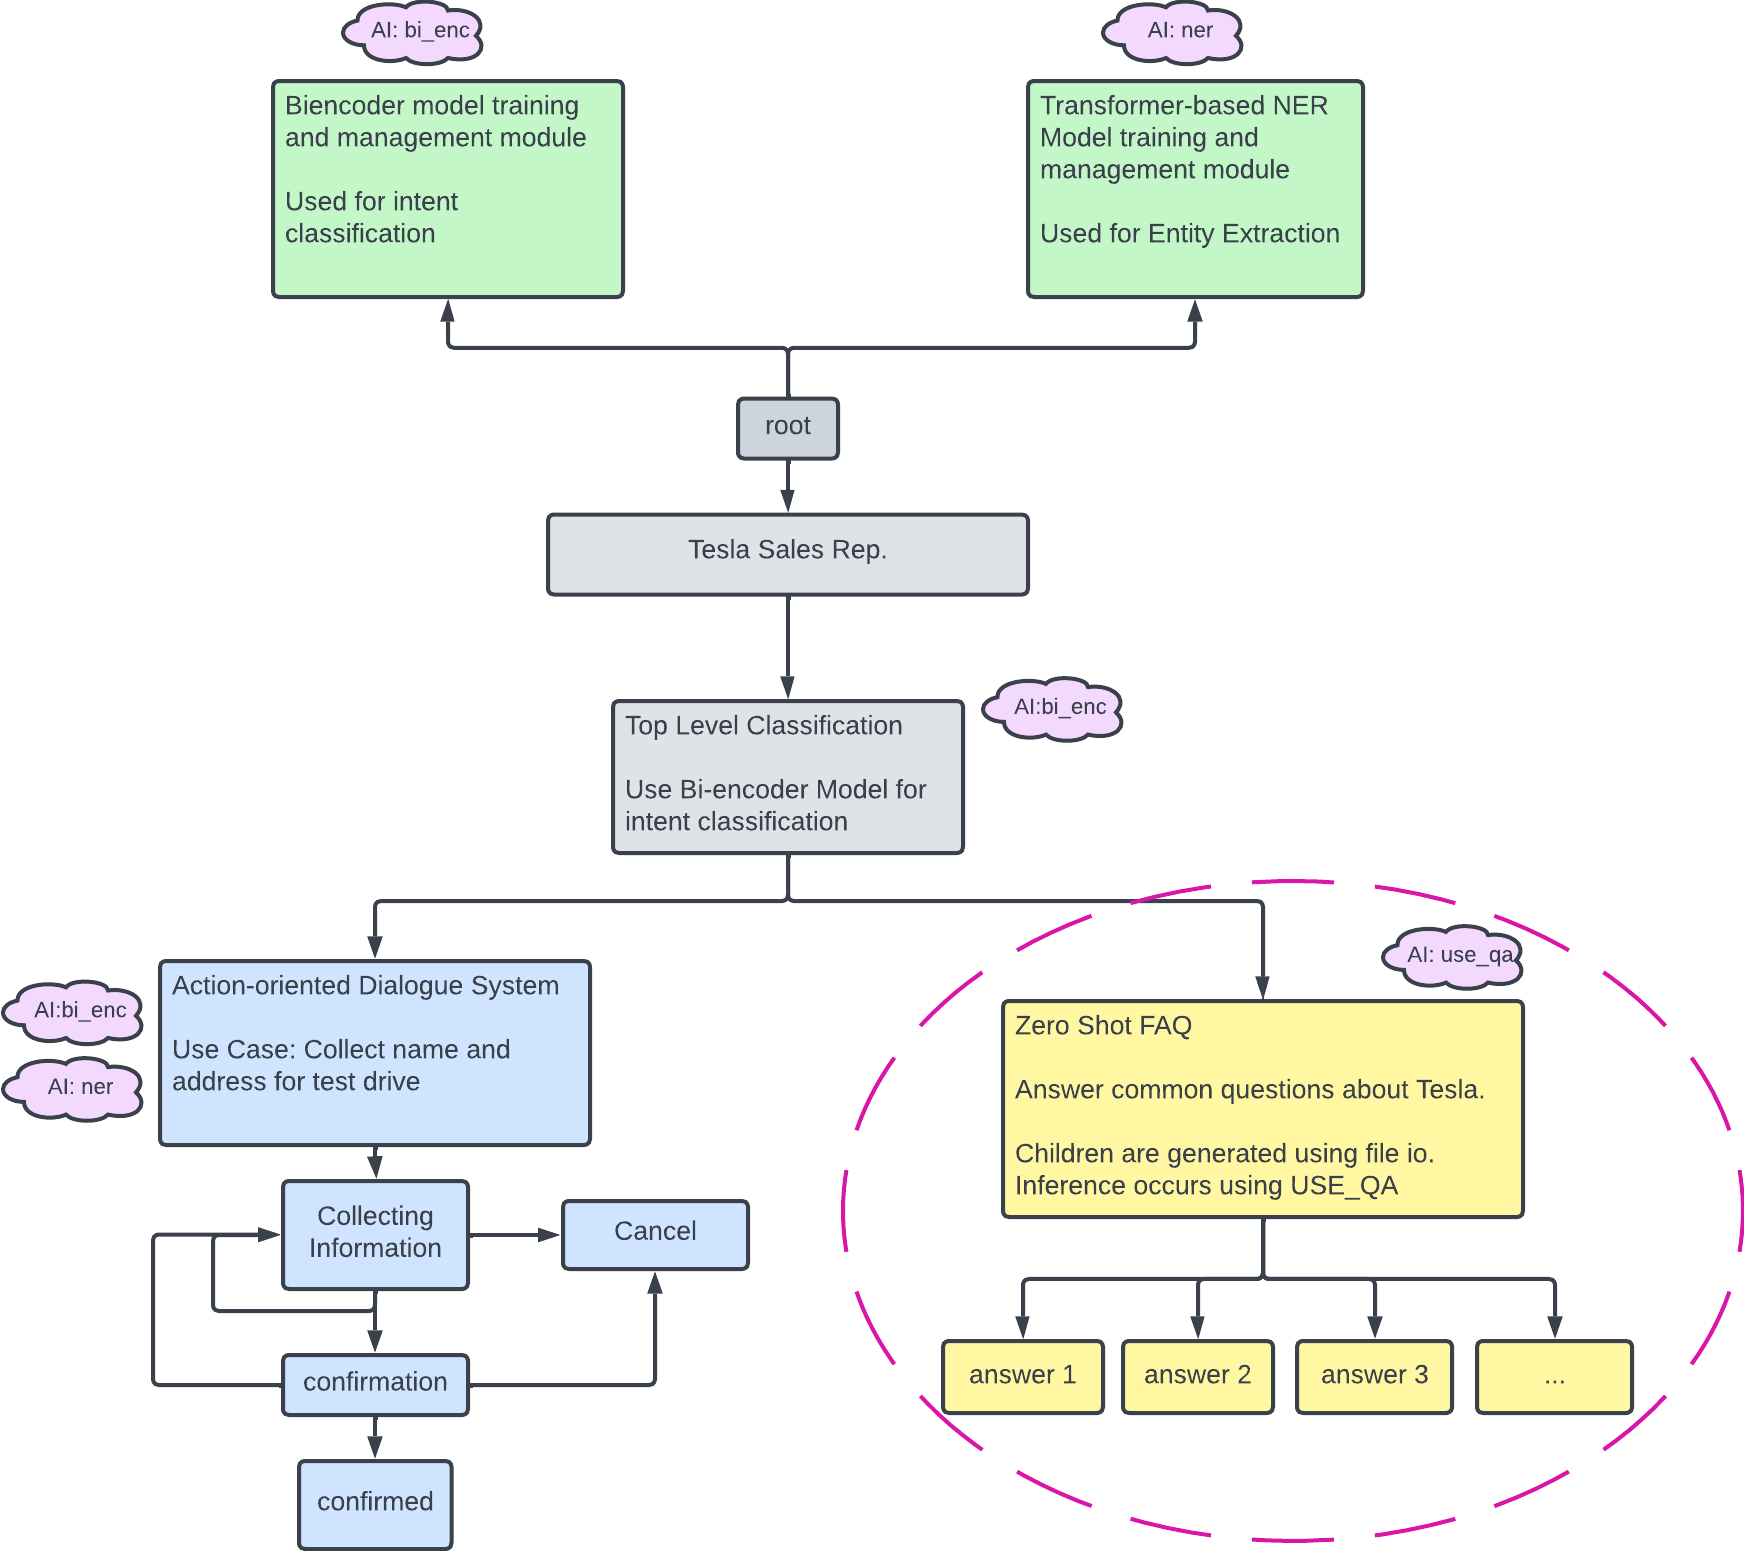
\includegraphics{images/arch.png}
\caption{Full architecture of Tesla AI}
\end{figure}

Here is a preview on what's next to come in this journey!

On the right is the architecture diagram of the complete system we are
going to build. Here are the major components:

\begin{itemize}
\tightlist
\item
  Zero-shot FAQ (what we have built so far).
\item
  Action-oriented Multi-turn Dialogue System.
\item
  Training and inference with an intent classification model.
\item
  Training and inference with an entity extraction model.
\item
  Testing.
\item
  Deploying your Jac application to a production environment.
\item
  Training data collection and curation.
\end{itemize}

\hypertarget{a-multi-turn-action-oriented-dialogue-system}{%
\section{A Multi-turn Action-oriented Dialogue
System}\label{a-multi-turn-action-oriented-dialogue-system}}

\hypertarget{introduction}{%
\subsection{Introduction}\label{introduction}}

In the previous section, we built a FAQ chabot. It can search in a
knowledge base of answers and find the most relevant one to a user's
question. While ths covers many diverse topics, certain user request can
not be satisfied by a single answer. For example, you might be looking
to open a new bank account which requires mulitple different pieces of
information about you. Or, you might be making a reservation at a
restaurant which requires information such as date, time and size of
your group. We refer to these as action-oriented conversational AI
requests, as they often lead to a certain action or objective.

When interacting with a real human agent to accomplish this type of
action-oriented requests, the interaction can get messy and unscripted
and it also varies from person to person. Again, use the restaurant
reservation as an example, one migh prefer to follow the guidance of the
agent and provide one piece of information at a time, while others might
prefer to provide all the neccessary information in one sentence at the
beginning of the interaction.

Therefore, in order to build a robust and flexible conversational AI to
mimic a real human agent to support these types of messy action-oriented
requests, we are going to need an architecture that is different than
the single-turn FAQ.

And that is what we are going to build in this section -- a multi-turn
action-oriented dialogue system.

\begin{quote}
\textbf{Warning}

Create a new jac file (\passthrough{\lstinline!dialogue.jac!}) before
moving forward. We will keep this program separate from the FAQ one we
built. But, KEEP the FAQ jac file around, we will integrate these two
systems into one unified conversational AI system later.
\end{quote}

\hypertarget{state-graph}{%
\subsection{State Graph}\label{state-graph}}

Let's first go over the graph architecture for the dialogue system. We
will be building a state graph. In a state graph, each node is a
conversational state, which represents a possible user state during a
dialgoue. The state nodes are connected with transition edges, which
encode the condition required to hop from one state to another state.
The conditions are often based on the user's input.

\hypertarget{define-the-state-nodes}{%
\subsection{Define the State Nodes}\label{define-the-state-nodes}}

We will start by defining the node types.

\begin{lstlisting}
node dialogue_root;

node dialogue_state {
    has name;
    has response;
}
\end{lstlisting}

Here we have a \passthrough{\lstinline!dialogue\_root!} as the entry
point to the dialogue system and multiple
\passthrough{\lstinline!dialogue\_state!} nodes representing the
conversational states. These nodes will be connected with a new type of
edge \passthrough{\lstinline!intent\_transition!}.

\hypertarget{custom-edges}{%
\subsection{Custom Edges}\label{custom-edges}}

\begin{lstlisting}
edge intent_transition {
    has intent;
}
\end{lstlisting}

This is the first custom edge we have introduced. In jac, just like
nodes, you can define custom edge types. Edges are also allowed
\passthrough{\lstinline!has!} variables.

In this case, we created an edge for intent transition. This is a state
transition that will be triggered conditioned on its intent being
detected from the user's input question.

\begin{quote}
\textbf{Note}

Custom edge type and variables enable us to encode information into
edges in addition to nodes. This is crucial for building a robust and
flexible graph.
\end{quote}

\hypertarget{build-the-graph-1}{%
\subsection{Build the graph}\label{build-the-graph-1}}

Let's build the first graph for the dialogue system.

\begin{lstlisting}
graph dialogue_system {
    has anchor dialogue_root;
    spawn {
        dialogue_root = spawn node::dialogue_root;
        test_drive_state = spawn node::dialogue_state(
            name = "test_drive",
            response = "Your test drive is scheduled for Jan 1st, 2023."
        );
        how_to_order_state = spawn node::dialogue_state (
            name = "how_to_order",
            response = "You can order a Tesla through our design studio."
        );

        dialogue_root -[intent_transition(intent="test drive")]-> test_drive_state;
        dialogue_root -[intent_transition(intent="order a tesla")]-> how_to_order_state;
    }
}
\end{lstlisting}

We have already covered the syntax for graph definition, such as the
\passthrough{\lstinline!anchor!} node and the
\passthrough{\lstinline!spawn!} block in the previous section. Refer to
the FAQ graph definition step if you need a refresher.

We have a new language syntax here
\passthrough{\lstinline!dialogue\_root -[intent\_transition(intent="test drive")]-> test\_drive\_state;!}.
Let's break this down! * If you recall, we have used a similar but
simpler syntax to connect two nodes with an edge
\passthrough{\lstinline!faq\_root --> faq\_state;!}. This connect
\passthrough{\lstinline!faq\_root!} to
\passthrough{\lstinline!faq\_state!} with a \textbf{generic} edge
pointing to \passthrough{\lstinline!faq\_state!}; * In
\passthrough{\lstinline!dialogue\_root -[intent\_transition(intent="test drive")]-> test\_drive\_state;!},
we are connecting the two states with a \textbf{custom} edge of the type
\passthrough{\lstinline!intent\_transition!}. * In addition, we are
initializing the variable \passthrough{\lstinline!intent!} of the edge
to be \passthrough{\lstinline!test drive!}.

To summarize, with this graph, a user will start at the dialogue root
state when they first start the conversation. Then based on the user's
question and its intent, we will

\hypertarget{initialize-the-graph-1}{%
\subsection{Initialize the graph}\label{initialize-the-graph-1}}

Let's create an \passthrough{\lstinline!init!} walker to for this new
jac program.

\begin{lstlisting}
walker init {
    root {
        spawn here ++> graph::dialogue_system;
    }
}
\end{lstlisting}

Put all the code so far in a new file and name it
\passthrough{\lstinline!dialogue.jac!}.

Let's initialize the graph and visualize it.

\begin{lstlisting}[language=bash]
jaseci > jac dot dialogue.jac
\end{lstlisting}

\begin{lstlisting}
strict digraph root {
    "n0" [ id="7b4ee7198c5b4dcd8acfcf739d6971fe", label="n0:root"  ]
    "n1" [ id="7caf939cfbce40d4968d904052368f30", label="n1:dialogue_root"  ]
    "n2" [ id="2e06be95aed449b59056e07f2077d854", label="n2:dialogue_state"  ]
    "n3" [ id="4aa3e21e13eb4fb99926a465528ae753", label="n3:dialogue_state"  ]
    "n1" -> "n3" [ id="6589c6d0dd67425ead843031c013d0fc", label="e0:intent_transition" ]
    "n1" -> "n2" [ id="f4c9981031a7446b855ec91b89aaa5ee", label="e1:intent_transition" ]
    "n0" -> "n1" [ id="bec764e7ee4048898799c2a4f01b9edb", label="e2" ]
}
\end{lstlisting}

\begin{figure}
\centering
\includegraphics{images/dialogue/dot_1.png}
\caption{DOT of the dialogue system}
\end{figure}

\hypertarget{build-the-walker-logic}{%
\subsection{Build the Walker Logic}\label{build-the-walker-logic}}

Let's now start building the walker to interact with this dialogue
system.

\begin{lstlisting}
walker talk {
    has question;
    root {
        question = std.input("> ");
        take --> node::dialogue_root;
    }
    dialogue_root {
        take -[intent_transition(intent==question)]-> node::dialogue_state;
    }
    dialogue_state {
        std.out(here.response);
    }
}
\end{lstlisting}

Similar to the first walker we built for the FAQ system, we are starting
with a simple string matching algorithm. Let's update the init walker to
include this walker.

\begin{lstlisting}
walker init {
    root {
        spawn here ++> graph::dialogue_system;
        spawn here walker::talk;
    }
}
\end{lstlisting}

Try out the following interactions

\begin{lstlisting}[language=bash]
$ jsctl jac run dialogue.jac
> test drive
Your test drive is scheduled for Jan 1st, 2023.
{
  "success": true,
  "report": [],
  "final_node": "urn:uuid:9b8d9e1e-d7fb-4e6e-ae86-7ef7c7ad28a7",
  "yielded": false
}
\end{lstlisting}

and

\begin{lstlisting}[language=bash]
$ jsctl jac run dialogue.jac
> order a tesla
You can order a Tesla through our design studio.
{
  "success": true,
  "report": [],
  "final_node": "urn:uuid:168590aa-d579-4f22-afe7-da75ab7eefa3",
  "yielded": false
}
\end{lstlisting}

What is happening here is based on the user's question, we are
traversing the corresponding dialogue state and then return the response
of that state. For now, we are just matching the incoming question with
the intent label as a simple algorithm, which we will now replace with
an AI model.

\begin{quote}
\textbf{Note}

Notice we are running \passthrough{\lstinline!jsctl!} commands directly
from the terminal without first entering the jaseci shell? Any
\passthrough{\lstinline!jsctl!} commands can be launched directly from
the terminal by just prepending it with \passthrough{\lstinline!jsctl!}.
Try it with the other \passthrough{\lstinline!jsctl!} comamnds we have
encountered so far, such as \passthrough{\lstinline!jac dot!}.
\end{quote}

\hypertarget{intent-classificaiton-with-bi-encoder}{%
\subsection{Intent classificaiton with
Bi-encoder}\label{intent-classificaiton-with-bi-encoder}}

Let's introduce an intent classification AI model. Intent Classification
is the task of detecting and assigning an intent to a given piece of
text from a list of pre-defined intents, to summarize what the text is
conveying or asking. It's one of the fundamental tasks in Natural
Language Processing (NLP) with broad applications in many areas.

There are many models that have been proposed and applied to intent
classification. For this tutorial, we are going to use a Bi-Encoder
model. A Bi-encoder model has two transformer-based encoders that each
encodes the input text and candidate intent labels into embedding
vectors and then the model compare the similarity between the embedding
vectors to find the most relevant/fitting intent label.

\begin{quote}
\textbf{Note}

If you don't fully understand the Bi-encoder model yet, do not worry! We
will provide the neccessary code and tooling for you to wield this model
as a black box. But, if you are interested, here is a paper for you to
read up on it https://arxiv.org/pdf/1908.10084.pdf!
\end{quote}

Now let's train the model. We have created a jac program and sample
training data for this. They are in the \passthrough{\lstinline!code!}
directory next to this tutorial. Copy
\passthrough{\lstinline!bi\_enc.jac!} and
\passthrough{\lstinline!clf\_train\_1.json!} to your working directory.

Let's first load the Bi-encoder action library into Jaseci.

\begin{lstlisting}[language=bash]
$ jsctl
jaseci > actions load module jaseci_ai_kit.bi_enc
\end{lstlisting}

We have provided an example training file that contains some starting
point training data for the two intents,
\passthrough{\lstinline!test drive!} and
\passthrough{\lstinline!order a tesla!}.

\begin{lstlisting}
jaseci > jac run bi_enc.jac -walk train -ctx "{\"train_file\": \"clf_train_1.json\"}"
\end{lstlisting}

We are still using \passthrough{\lstinline!jac run!} but as you have
noticed, this time we are using some new arguments. So let's break it
down. * \passthrough{\lstinline!-walk!} specifies the name of the walker
to run. By default, it runs the \passthrough{\lstinline!init!} walker. *
\passthrough{\lstinline!-ctx!} stands for
\passthrough{\lstinline!context!}. This lets us provide input parameters
to the walker. The input parameters are defined as
\passthrough{\lstinline!has!} variables in the walker.

\begin{quote}
\textbf{Warning}

\passthrough{\lstinline!-ctx!} expects a json string that contains a
dictionary of parameters and their values. Since we are running this on
the command line, you will need to escape the quotation marks
\passthrough{\lstinline!"!} properly for it to be a valid json string.
Pay close attention to the example here
\passthrough{\lstinline!-ctx "\{\\"train\_file\\": \\"clf\_train\_1.json\\"\}"!}
and use this as a reference.
\end{quote}

You should see an output block that looks like the following repeating
many times on your screen:

\begin{lstlisting}[language=bash]
...
Epoch : 5
loss : 0.10562849541505177
LR : 0.0009854014598540146
...
\end{lstlisting}

Each training epoch, the above output will print with the training loss
and learning rate at that epoch. By default, the model is trained for 50
epochs.

If the training successfully finishes, you should see
\passthrough{\lstinline!"success": true!} at the end.

Now that the model has finished training, let's try it out! You can use
the \passthrough{\lstinline!infer!} walker to play with the model and
test it out! \passthrough{\lstinline!infer!} is short for inference,
which means using a trained model to run prediction on a given input.

\begin{lstlisting}[language=bash]
jaseci > jac run bi_enc.jac -walk infer -ctx "{\"labels\": [\"test drive\", \"order a tesla\"]}"
\end{lstlisting}

Similar to training, we are using \passthrough{\lstinline!jac run!} to
specifically invoke the \passthrough{\lstinline!infer!} walker and
provide it with custom parameters. The custom paremeter is the list of
candidate intent labels, which are \passthrough{\lstinline!test drive!}
and \passthrough{\lstinline!order a tesla!} in this case, as these were
the intents the model was trained on.

\begin{lstlisting}[language=bash]
jaseci > jac run bi_enc.jac -walk infer -ctx "{\"labels\": [\"test drive\", \"order a tesla\"]}"
Enter input text (Ctrl-C to exit)> i want to order a tesla
{"label": "order a tesla", "score": 9.812651595405981}
Enter input text (Ctrl-C to exit)> i want to test drive
{"label": "test drive", "score": 6.931458692617463}
Enter input text (Ctrl-C to exit)>
\end{lstlisting}

In the output here, \passthrough{\lstinline!label!} is the predicted
intent label and \passthrough{\lstinline!score!} is the score assigned
by the model to that intent.

\begin{quote}
\textbf{Note}

One of the advantage of the bi-encoder model is that candidate intent
labels can be dynamically defined at inference time, post training. This
enables us to create custom contextual classifiers situationally from a
single trained model. We will leverage this later as our dialogue system
becomes more complex.
\end{quote}

Congratulations! You just trained your first intent classifier, easy as
that.

The trained model is kept in memory and active until they are explicitly
saved with \passthrough{\lstinline!save\_model!}. To save the trained
model to a location of your choosing, run

\begin{lstlisting}[language=bash]
jaseci > jac run bi_enc.jac -walk save_model -ctx "{\"model_path\": \"dialogue_intent_model\"}"
\end{lstlisting}

Similarly, you can load a saved model with
\passthrough{\lstinline!load\_model!}

\begin{lstlisting}[language=bash]
jaseci > jac run bi_enc.jac -walk load_model -ctx "{\"model_path\": \"dialogue_intent_model\"}"
\end{lstlisting}

Always remember to save your trained models!

\begin{quote}
\textbf{Warning}

\passthrough{\lstinline!save\_model!} works with relative path. When a
relative model path is specified, it will save the model at the location
relative to \textbf{location of where you run jsctl}. Note that until
the model is saved, the trained weights will stay in memory, which means
that it will not persisit between \passthrough{\lstinline!jsctl!}
session. So once you have a trained model you like, make sure to save
them so you can load them back in the next jsctl session.
\end{quote}

\hypertarget{integrate-the-intent-classifier}{%
\subsection{Integrate the Intent
Classifier}\label{integrate-the-intent-classifier}}

Now let's update our walker to use the trained intent classifier.

\begin{lstlisting}
walker talk {
    has question;
    can bi_enc.infer;
    root {
        question = std.input("> ");
        take --> node::dialogue_root;
    }
    dialogue_root {
        intent_labels = -[intent_transition]->.edge.intent;
        predicted_intent = bi_enc.infer(
            contexts = [question],
            candidates = intent_labels,
            context_type = "text",
            candidate_type = "text"
        )[0]["predicted"]["label"];
        take -[intent_transition(intent==predicted_intent)]-> node::dialogue_state;
    }
    dialogue_state {
        std.out(here.response);
    }
}
\end{lstlisting}

\passthrough{\lstinline!intent\_labels = -[intent\_transition]->.edge.intent!}
collects the \passthrough{\lstinline!intent!} variables of all the
outgoing \passthrough{\lstinline!intent\_transition!} edges. This
represents the list of candidate intent labels for this state.

Try playing with different questions, such as

\begin{lstlisting}[language=bash]
$ jsctl
jaseci > jac run dialogue.jac
> hey yo, I heard tesla cars are great, how do i get one?
You can order a Tesla through our design studio.
{
  "success": true,
  "report": [],
  "final_node": "urn:uuid:af667fdf-c2b0-4443-9ccd-7312bc4c66c4",
  "yielded": false
}
\end{lstlisting}

\hypertarget{making-our-dialogue-system-multi-turn}{%
\subsection{Making Our Dialogue System
Multi-turn}\label{making-our-dialogue-system-multi-turn}}

Dialogues in real life have many turn of interaction. Our dialogue
system should also support that to provide a human-like conversational
experinece. In this section, we are going to take the dialogue system to
the next level and create a multi-turn dialogue experience.

Before we do that we need to introduce two new concepts in Jac: node
abilities and inheritance.

\hypertarget{node-abilities}{%
\subsubsection{Node Abilities}\label{node-abilities}}

Node abilities are code that encoded as part of each node type. They
often contain logic that read, write and generally manipulate the
variables and states of the nodes. Node abilities are defined with the
\passthrough{\lstinline!can!} keyword inside the definition of nodes,
for example, in the code below,
\passthrough{\lstinline!get\_plate\_number!} is an ability of the
\passthrough{\lstinline!vehicle!} node.

\begin{lstlisting}
node vehicle {
    has plate_numer;
    can get_plate_numer {
        report here.plate_number;
    }
}
\end{lstlisting}

To learn more about node abilities, refer to the relevant sections of
the Jaseci Bible. \textgreater{} \textbf{Note} \textgreater{}
\textgreater{} Node abilities look and function similarly to member
functions in object-oriented programming (OOP). However, there is a key
difference in the concepts. Node abilities are the key concept in
data-spatial programming, where the logic should stay close to its
working set data in terms of the programming syntax.

\hypertarget{inheritance}{%
\subsubsection{Inheritance}\label{inheritance}}

Jac supports inheritance for nodes and edges. Node variables (defined
with \passthrough{\lstinline!has!}) and node abilities (defined with
\passthrough{\lstinline!can!}) are inherited and can be overwritten by
children nodes.

Here is an example:

\begin{lstlisting}
node vehicle {
    has plate_number;
    can get_plate_number {
        report here.plate_number;
    }
}

node car:vehicle {
    has plate_number = "RAC001";
}

node bus:vehicle {
    has plate_number = "SUB002";
}
\end{lstlisting}

To learn more about inheritance in Jac, refer to the relevant sections
of the Jaseci Bible.

\hypertarget{build-the-multi-turn-dialogue-graph}{%
\subsection{Build the Multi-turn Dialogue
Graph}\label{build-the-multi-turn-dialogue-graph}}

Now that we have learnt about node abilities and node inheritance, let's
put these new concepts to use to build a new graph for the multi-turn
dialogue system

There are multiple parts to this so let's break it down one by one

\hypertarget{dialogue-state-specific-logic}{%
\subsubsection{Dialogue State Specific
Logic}\label{dialogue-state-specific-logic}}

With the node abilities and node inheritance, we will now introduce
state specific logic. Take a look at how the
\passthrough{\lstinline!dialogue\_root!} node definition has changed.

\begin{lstlisting}
node dialogue_state {
    can bi_enc.infer;
    can tfm_ner.extract_entity;

    can classify_intent {
        intent_labels = -[intent_transition]->.edge.intent;
        visitor.wlk_ctx["intent"] = bi_enc.infer(
            contexts = [visitor.question],
            candidates = intent_labels,
            context_type = "text",
            candidate_type = "text"
        )[0]["predicted"]["label"];
    }

    can extract_entities {
        // Entity extraction logic will be added a bit later on.
    }

    can init_wlk_ctx {
        new_wlk_ctx = {
            "intent": null,
            "entities": {},
            "prev_state": null,
            "next_state": null,
            "respond": false
        };
        if ("entities" in visitor.wlk_ctx) {
            // Carry over extracted entities from previous interaction
            new_wlk_ctx["entities"] = visitor.wlk_ctx["entities"];
        }
        visitor.wlk_ctx = new_wlk_ctx;
    }
    can nlu {}
    can process {
        if (visitor.wlk_ctx["prev_state"]): visitor.wlk_ctx["respond"] = true;
        else {
            visitor.wlk_ctx["next_state"] = net.root();
            visitor.wlk_ctx["prev_state"] = here;
        }
    }
    can nlg {}
}

node dialogue_root:dialogue_state {
    has name = "dialogue_root";
    can nlu {
        ::classify_intent;
    }
    can process {
        visitor.wlk_ctx["next_state"] = (-[intent_transition(intent==visitor.wlk_ctx["intent"])]->)[0];
    }
    can nlg {
        visitor.response = "Sorry I can't handle that just yet. Anything else I can help you with?";
    }
}
\end{lstlisting}

There are many interesting things going on in these \textasciitilde30
lines of code so let's break it down! * The
\passthrough{\lstinline!dialogue\_state!} node is the parent node and it
is similar to a virtual class in OOP. It defines the variables and
abilities of the nodes but the details of the abilities will be
specified in the inheriting children nodes. * In this case,
\passthrough{\lstinline!dialogue\_state!} has 4 node abilities: *
\passthrough{\lstinline!can nlu!}: NLU stands for Natural Language
Understanding. This ability will analyze user's incoming requset and
apply AI models. * \passthrough{\lstinline!can process!}: This ability
uses the NLU results and figure out the next dialogue state the walker
should go to. * \passthrough{\lstinline!can nlg!}: NLG stands for
Natural Language Generation. This abilitiy will compose response to the
user, often based on the results from \passthrough{\lstinline!nlu!}. *
\passthrough{\lstinline!can classify\_intent!}: an ability to handle
intent classification. This is the same intent classification logic that
has been copied over from the walker. *
\passthrough{\lstinline!can extract\_entities!}: a new ability with a
new AI model -- entity extraction. We will cover that just in a little
bit (read on!). * Between these four node abilities,
\passthrough{\lstinline!classify\_intent!} and
\passthrough{\lstinline!extract\_entities!} have concrete logic defined
while \passthrough{\lstinline!nlu!} and \passthrough{\lstinline!nlg!}
are ``virtual node abilities'', which will be specified in each of the
inheriting children. * For example,
\passthrough{\lstinline!dialogue\_root!} inherit from
\passthrough{\lstinline!dialogue\_state!} and overwrites
\passthrough{\lstinline!nlu!} and \passthrough{\lstinline!nlg!}: * for
\passthrough{\lstinline!nlu!}, it invokes intent classification because
it needs to decide what's the intent of the user (test drive vs order a
tesla). * for \passthrough{\lstinline!nlg!}, it just has a general
fall-back response in case the system can't handle user's ask. *
\textbf{New Syntax}: \passthrough{\lstinline!visitor!} is the walker
that is ``visiting'' the node. And through
\passthrough{\lstinline!visitor.*!}, the node abilities can access and
update the context of the walker. In this case, the node abilities are
updating the \passthrough{\lstinline!response!} variable in the walker's
context so that the walker can return the response to its caller, as
well as the \passthrough{\lstinline!wlk\_ctx!} variable that will
contain various walker context as the walker traverse the graph. * the
\passthrough{\lstinline!init\_wlk\_ctx!} ability initializes the
\passthrough{\lstinline!wlk\_ctx!} variable for each new question.

In this new node architecture, each dialogue state will have its own
node type, specifying their state-specific logic in
\passthrough{\lstinline!nlu!}, \passthrough{\lstinline!nlg!} and
\passthrough{\lstinline!process!}. Let's take a look!

\begin{lstlisting}
node how_to_order_state:dialogue_state {
    has name = "how_to_order";
    can nlg {
        visitor.response = "You can order a Telsa through our design studio";
    }
}

node test_drive_state:dialogue_state {
    has name = "test_drive";
    can nlu {
        if (!visitor.wlk_ctx["intent"]): ::classify_intent;
        ::extract_entities;
    }
    can process {
        // Check entity transition
        required_entities = -[entity_transition]->.edge[0].context["entities"];
        if (vector.sort_by_key(visitor.wlk_ctx["entities"].d::keys) == vector.sort_by_key(required_entities)) {
            visitor.wlk_ctx["next_state"] = -[entity_transition]->[0];
            visitor.wlk_ctx["prev_state"] = here;
        } elif (visitor.wlk_ctx["prev_state"] and !visitor.wlk_ctx["prev_state"].context["name"] in ["test_drive", "td_confirmation"]){
            next_state = -[intent_transition(intent==visitor.wlk_ctx["intent"])]->;
            if (next_state.length > 0 and visitor.wlk_ctx["intent"] != "no") {
                visitor.wlk_ctx["next_state"] = next_state[0];
                visitor.wlk_ctx["prev_state"] = here;
            } else {
                visitor.wlk_ctx["respond"] = true;
            }
        } else {
            visitor.wlk_ctx["respond"] = true;
        }
    }
    can nlg {
        if ("name" in visitor.wlk_ctx["entities"] and "address" not in visitor.wlk_ctx["entities"]):
            visitor.response = "What is your address?";
        elif ("address" in visitor.wlk_ctx["entities"] and "name" not in visitor.wlk_ctx["entities"]):
            visitor.response = "What is your name?";
        else:
            visitor.response = "To set you up with a test drive, we will need your name and address.";
    }
}

node td_confirmation:dialogue_state {
    has name = "test_drive_confirmation";
    can nlu {
        if (!visitor.wlk_ctx["intent"]): ::classify_intent;
    }
    can process {
        if (visitor.wlk_ctx["prev_state"]): visitor.wlk_ctx["respond"] = true;
        else {
            visitor.wlk_ctx["next_state"] = -[intent_transition(intent==visitor.wlk_ctx["intent"])]->[0];
            visitor.wlk_ctx["prev_state"] = here;
        }
    }
    can nlg {
        visitor.response =
            "Can you confirm your name to be " + visitor.wlk_ctx["entities"]["name"][0] + " and your address as " + visitor.wlk_ctx["entities"]["address"][0] + "?";
    }
}

node td_confirmed:dialogue_state {
    has name = "test_drive_confirmed";
    can nlg {
        visitor.response = "You are all set for a Tesla test drive!";
    }
}

node td_canceled:dialogue_state {
    has name = "test_drive_canceled";
    can nlg {
        visitor.response = "No worries. We look forward to hearing from you in the future!";
    }
}
\end{lstlisting}

\begin{itemize}
\tightlist
\item
  Each dialogue state now has its own node type, all inheriting from the
  same generic \passthrough{\lstinline!dialogue\_state!} node type.
\item
  We have 4 dialogue states here for the test drive capability:

  \begin{itemize}
  \tightlist
  \item
    \passthrough{\lstinline!test\_drive!}: This is the main state of the
    test drive intent. It is responsible for collecting the neccessary
    information from the user.
  \item
    \passthrough{\lstinline!test\_drive\_confirmation!}: Ths is the
    state for user to confirm the information they have provided are
    correct and is ready to actually schedule the test drive.
  \item
    \passthrough{\lstinline!test\_drive\_confirmed!}: This is the state
    after the user has confirmed.
  \item
    \passthrough{\lstinline!test\_drive\_canceled!}: User has decided,
    in the middle of the dialogue, to cancel their request to schedule a
    test drive.
  \end{itemize}
\item
  The \passthrough{\lstinline!process!} ability contains the logic that
  defines the conversational flow of the dialogue system. It uses the
  data in \passthrough{\lstinline!wlk\_ctx!} and assign a
  \passthrough{\lstinline!next\_state!} which will be used by the walker
  in a \passthrough{\lstinline!take!} statement, as you will see in a
  just a little bit.
\item
  \textbf{New Syntax}: The code in
  \passthrough{\lstinline!test\_drive\_state!}'s ability demonstrates
  jac support for list and dictionary. To access the list and
  dictionary-specific functions, first cast the variable with
  \passthrough{\lstinline!.l!}/\passthrough{\lstinline!.list!} for list
  and \passthrough{\lstinline!.d!}/\passthrough{\lstinline!.dict!} for
  dictionaries, then proceed with \passthrough{\lstinline!:!} to access
  the built-in functions for list and dictioinaries. For more on jac's
  built-in types, refer to the relevant sections of the Jaseci Bible.

  \begin{itemize}
  \tightlist
  \item
    Specifically in this case, we are comparing the list of entities of
    the \passthrough{\lstinline!entity\_transition!} edge with the list
    of entities that have been extracted by the walker and the AI model
    (stored in \passthrough{\lstinline!wlk\_ctx["entities]!}). Since
    there can be multiple entities required and they can be extracted in
    arbitrary order, we are sorting and then comparing here.
  \end{itemize}
\item
  \textbf{New Syntax}:
  \passthrough{\lstinline!-[entity\_transition]->.edge!} shows how to
  access the edge variable. Consider
  \passthrough{\lstinline!-[entity\_transition]->!} as a filter. It
  returns all valid nodes that are connected to the implicit
  \passthrough{\lstinline!here!} via an
  \passthrough{\lstinline!entity\_transition!}. On its own, it will
  return all the qualified nodes. When followed by
  \passthrough{\lstinline!.edge!}, it will return the set of edges that
  are connected to the qualified nodes.
\end{itemize}

You might notice that some states do not have a
\passthrough{\lstinline!process!} ability. These are states that do not
have any outgoing transitions, which we refer to as leaf nodes. If these
nodes are reached, they indicate that a dialogue has been completed end
to end. The next state for these node will be returning to the root node
so that the next dialogue can start fresh. To facilitate this, we will
add the following logic to the \passthrough{\lstinline!process!} ability
of the \textbf{parent \passthrough{\lstinline!dialogue\_state!} node} so
that by default, any nodes inheriting it will follow this rule.

\begin{lstlisting}
node dialogue_state {
...
    can process {
        if (visitor.wlk_ctx["prev_state"]): visitor.wlk_ctx["respond"] = true;
        else {
            visitor.wlk_ctx["next_state"] = net.root();
            visitor.wlk_ctx["prev_state"] = here;
        }
    }
...
}
\end{lstlisting}

\begin{quote}
\textbf{Note}

Pay attention to the 4 dialogue states here. This pattern of
\passthrough{\lstinline!main!} -\textgreater{}
\passthrough{\lstinline!confirmation!} -\textgreater{}
\passthrough{\lstinline!confirmed!} -\textgreater{}
\passthrough{\lstinline!canceled!} is a very common conversational state
graph design pattern and can apply to many topics, e.g., make a
restaurant reservation and opening a new bank account. Essentially,
almost any action-oriented requests can leverage this conversational
pattern. Keep this in mind!
\end{quote}

\hypertarget{entity-extraction}{%
\subsubsection{Entity Extraction}\label{entity-extraction}}

Previously, we have introduced intent classification and how it helps to
build a dialogue system. We now introduce the second key AI models, that
is specifically important for a multi-turn dialogue system, that is
entity/slot extraction.

Entity extraction is a NLP task that focuses on extracting words or
phrases of interests, or entities, from a given piece of text. Entity
extraction, sometimes also referred to as Named Entity Recognition
(NER), is useful in many domains, including information retrieval and
conversational AI. We are going to use a transformer-based entity
extraction model for this exercise.

Let's first take a look at how we are going to use an entity model in
our program. Then we will work on training an entity model.

First, we introduce a new type of transition:

\begin{lstlisting}
edge entity_transition {
    has entities;
}
\end{lstlisting}

Recall the \passthrough{\lstinline!intent\_transition!} that will
trigger if the intent is the one that is being predicted. Similarly, the
idea behind an \passthrough{\lstinline!entity\_transition!} is that we
will traverse this transition if all the specified entities have been
fulfilled, i.e., they have been extracted from user's inputs.

With the \passthrough{\lstinline!entity\_transition!}, let's update our
graph

\begin{lstlisting}
graph dialogue_system {
    has anchor dialogue_root;
    spawn {
        dialogue_root = spawn node::dialogue_root;
        test_drive_state = spawn node::test_drive_state;
        td_confirmation = spawn node::td_confirmation;
        td_confirmed = spawn node::td_confirmed;
        td_canceled = spawn node::td_canceled;

        how_to_order_state = spawn node::how_to_order_state;

        dialogue_root -[intent_transition(intent="test drive")]-> test_drive_state;
        test_drive_state -[intent_transition(intent="cancel")]-> td_canceled;
        test_drive_state -[entity_transition(entities=["name", "address"])]-> td_confirmation;
        test_drive_state -[intent_transition(intent="provide name or address")]-> test_drive_state;
        td_confirmation - [intent_transition(intent="yes")]-> td_confirmed;
        td_confirmation - [intent_transition(intent="no")]-> test_drive_state;
        td_confirmation - [intent_transition(intent="cancel")]-> td_canceled;

        dialogue_root -[intent_transition(intent="order a tesla")]-> how_to_order_state;
    }
}
\end{lstlisting}

Your graph should look something like this!

\begin{figure}
\centering
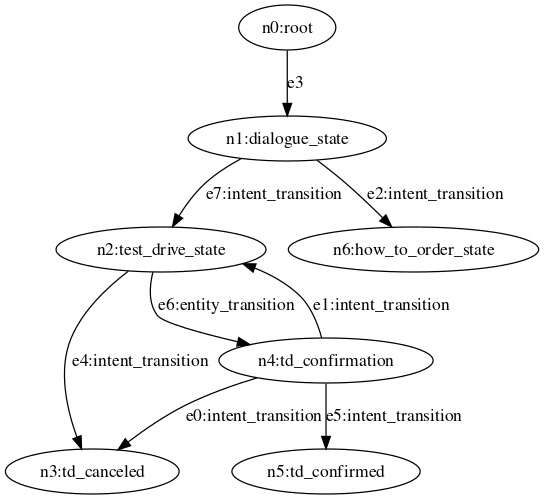
\includegraphics{images/dialogue/multi-turn.png}
\caption{Multi-turn Dialogue Graph}
\end{figure}

\hypertarget{update-the-walker-for-multi-turn-dialogue}{%
\subsection{Update the Walker for Multi-turn
Dialogue}\label{update-the-walker-for-multi-turn-dialogue}}

Let's now turn our focus to the walker logic

\begin{lstlisting}
walker talk {
    has question;
    has wlk_ctx = {};
    has response;
    root {
        take --> node::dialogue_root;
    }
    dialogue_state {
        if (!question) {
            question = std.input("Question (Ctrl-C to exit)> ");
            here::init_wlk_ctx;
        }
        here::nlu;
        here::process;
        if (visitor.wlk_ctx["respond"]) {
            here::nlg;
            std.out(response);
            question = null;
            take here;
        } else {
            take visitor.wlk_ctx["next_state"] else: take here;
        }
    }
}
\end{lstlisting}

The walker logic looks very different now. Let's break it down! * First
off, because the intent classification logic is now a node ability, the
walker logic has become simpler and, more importantly, more focused on
graph traversal logic without the detailed (and occasionally convoluted)
logic required to process to interact with an AI model. * \textbf{New
Syntax}: \passthrough{\lstinline!here::nlu!} and
\passthrough{\lstinline!here::nlg!} invokes the node abilities.
\passthrough{\lstinline!here!} can be subtitied with any node variables,
not just the one the walker is currently on.

Now that we have explained some of the new language syntax here, let's
go over the overall logic of this walker. For a new question from the
user, the walker will 1. analyze the question
(\passthrough{\lstinline!here:nlu!}) to identify its intent
(\passthrough{\lstinline!predicted\_intent!}) and/or extract its
entities (\passthrough{\lstinline!extracted\_entities!}). 2. based on
the NLU results, it will traverse the dialogue state graph (the two
\passthrough{\lstinline!take!} statements) to a new dialogue state 3. at
this new dialogue state, it will perform NLU, specific to that state
(recall that \passthrough{\lstinline!nlu!} is a node ability that varies
from node to node) and repeat step 2 4. if the walker can not make any
state traversal anymore (\passthrough{\lstinline!take ... else \{\}!}),
it will construct a response (\passthrough{\lstinline!here::nlg!}) using
the information it has gathered so far (the walker's context) and return
that response to the user.

If this still sounds fuzzy, don't worry! Let's use a real dialogue as an
example to illustrate this.

\begin{lstlisting}[language=bash]
Turn #1:
    User: hey i want to schedule a test drive
    Tesla AI: To set you up with a test drive, we will need your name and address.

Turn #2:
    User: my name is Elon and I live at 123 Main Street
    Tesla AI: Can you confirm your name to be Elon and your address as 123 Main Street?

Turn #3:
    User: Yup! that is correct
    Tesla AI: You are all set for a Tesla test drive!
\end{lstlisting}

At turn \#1, * The walker starts at
\passthrough{\lstinline!dialogue\_root!}. * The
\passthrough{\lstinline!nlu!} at
\passthrough{\lstinline!dialogue\_root!} is called and classify the
intent to be \passthrough{\lstinline!test drive!}. * There is an
\passthrough{\lstinline!intent\_transition(test\_drive)!} connecting
\passthrough{\lstinline!dialogue\_root!} to
\passthrough{\lstinline!test\_drive\_state!} so the walker
\passthrough{\lstinline!takes!} itself to
\passthrough{\lstinline!test\_drive\_state!} . * We are now at
\passthrough{\lstinline!test\_drive\_state!}, its
\passthrough{\lstinline!nlu!} requires
\passthrough{\lstinline!entity\_extraction!} which will look for
\passthrough{\lstinline!name!} and \passthrough{\lstinline!address!}
entities. In this case, neither is provided by the user. * As a result,
the walker can no longer traverse based on the
\passthrough{\lstinline!take!} rules and thus construct a response based
on the \passthrough{\lstinline!nlg!} logic at the
\passthrough{\lstinline!test\_drive\_state!}.

At turn \#2, * The walker starts at
\passthrough{\lstinline!test\_drive\_state!}, picking up where it left
off. * \passthrough{\lstinline!nlu!} at
\passthrough{\lstinline!test\_drive\_state!} perform intent
classification and entity extractions. This time it will pick up both
name and address. * As a result, the first
\passthrough{\lstinline!take!} statement finds a qualified path and take
that path to the \passthrough{\lstinline!td\_confirmation!} node. * At
\passthrough{\lstinline!td\_confirmation!}, no valid take path exists so
a response is returned.

\begin{quote}
\textbf{Note}

Turn \#3 works similiarly as turn \#1. See if you can figure out how the
walker reacts at turn \#3 yourself!
\end{quote}

\hypertarget{train-an-entity-extraction-model}{%
\subsection{Train an Entity Extraction
Model}\label{train-an-entity-extraction-model}}

Let's now train an entity extraction model! We are using a
transformer-based token classification model.

First, we need to load the actions. The action set is called
\passthrough{\lstinline!tfm\_ner!} (\passthrough{\lstinline!tfm!} stands
for transformer).

\begin{lstlisting}[language=bash]
jaseci > actions load module jaseci_ai_kit.tfm_ner
\end{lstlisting}

\begin{quote}
\textbf{Warning}

If you installed \passthrough{\lstinline!jaseci\_ai\_kit!} prior to
September 5th, 2022, please upgrade via
\passthrough{\lstinline!pip install --upgrade jaseci\_ai\_kit!}. There
has been an update to the module that you will need for remainder of
this exercise. You can check your installed version via
\passthrough{\lstinline!pip show jaseci\_ai\_kit!}. You need to be on
version 1.3.4.6 or higher.
\end{quote}

Similar to Bi-encoder, we have provided a jac program to train and
inference with this model, as well as an example training dataset. Go
into the \passthrough{\lstinline!code/!} directory and copy
\passthrough{\lstinline!tfm\_ner.jac!} and
\passthrough{\lstinline!ner\_train.json!} to your working directory. We
are training the model to detect two entities,
\passthrough{\lstinline!name!} and \passthrough{\lstinline!address!},
for the test drive use case.

Let's quickly go over the training data format.

\begin{lstlisting}
[
    "sure my name is [tony stark](name) and i live at [10880 malibu point california](address)",
    "my name is [jason](name)"
]
\end{lstlisting}

The training data is a json list of strings, each of which is a training
example. \passthrough{\lstinline![]!} indicate the entitiy text while
the \passthrough{\lstinline!()!} following it defines the entity type.
So in the example above, we have two entities,
\passthrough{\lstinline!name:tony stark!} and
\passthrough{\lstinline!address: 10880 malibu point california!}.

To train the model, run

\begin{lstlisting}[language=bash]
jaseci > jac run tfm_ner.jac -walk train -ctx "{\"train_file\": \"ner_train.json\"}"
\end{lstlisting}

After the model is finished training, you can play with the model using
the \passthrough{\lstinline!infer!} walker

\begin{lstlisting}
jaseci > jac run tfm_ner.jac -walk infer
\end{lstlisting}

For example,

\begin{lstlisting}[language=bash]
jaseci > jac run tfm_ner.jac -walk infer
Enter input text (Ctrl-C to exit)> my name is jason
[{"entity_text": "jason", "entity_value": "name", "conf_score": 0.5514775514602661, "start_pos": 11, "end_pos": 16}]
\end{lstlisting}

The output of this model is a list of dictionaries, each of which is one
detected entitiy. For each detected entity,
\passthrough{\lstinline!entity\_value!} is the type of entity, so in
this case either \passthrough{\lstinline!name!} or
\passthrough{\lstinline!address!}; and
\passthrough{\lstinline!entity\_text!} is the detected text from the
input for this entity, so in this case the user's name or their address.

Let's now update the node ability to use the entity model.

\begin{lstlisting}
node dialogue_state {
    ...
    can extract_entities {
        res = tfm_ner.extract_entity(visitor.question);
        for ent in res {
            ent_type = ent["entity_value"];
            ent_text = ent["entity_text"];
            if (!(ent_type in visitor.wlk_ctx["entities"])){
                visitor.wlk_ctx["entities"][ent_type] = [];
            }
            visitor.wlk_ctx["entities"][ent_type].l::append(ent_text);
        }
    }
    ...
}
\end{lstlisting}

There is one last update we need to do before this is fully functional.
Because we have more dialogue states and a more complex graph, we need
to update our classifier to include the new intents. We have provided an
example training dataset at
\passthrough{\lstinline!code/clf\_train\_2.json!}. Re-train the
bi-encoder model with this dataset.

\begin{quote}
\textbf{Note}

Refer to previous code snippets if you need a reminder on how to train
the bi-encoder classifier model.
\end{quote}

\begin{quote}
\textbf{Note}

Remember to save your new entity extraction model!
\end{quote}

Now try running the walker again with
\passthrough{\lstinline!jac run dialogue.jac!}!

Congratulations! You now have a fully functional multi-turn dialogue
system that can handle test drive requests!

\hypertarget{unify-the-dialogue-and-faq-systems}{%
\section{Unify the Dialogue and FAQ
Systems}\label{unify-the-dialogue-and-faq-systems}}

So far, we have built two separate conversational AI systems, a FAQ
system that automatically scales with the available question-answer
pairs and a multi-turn action-oriented dialogue system that can handle
complex requests. These two systems serve different use cases and can be
combined to a single system to provide a flexible and robust
conversational AI experience. In this section, we are going to unify
these two systems into one coherent conversational AI system.

While these two systems rely on different AI models, they share many of
the same logic flow. They both follow the general steps of first
analyizing user's question with NLU AI models, make decision on the next
conversational state to be and then construct and return a response to
the user. Leveraging this shared pattern, we will first unify the node
architecture of the two systems with a single parent node type,
\passthrough{\lstinline!cai\_state!} (\passthrough{\lstinline!cai!} is
short of conversational AI).

\begin{lstlisting}
node cai_state {
    has name;
    can init_wlk_ctx {
        new_wlk_ctx = {
            "intent": null,
            "entities": {},
            "prev_state": null,
            "next_state": null,
            "respond": false
        };
        if ("entities" in visitor.wlk_ctx) {
            // Carry over extracted entities from previous interaction
            new_wlk_ctx["entities"] = visitor.wlk_ctx["entities"];
        }
        visitor.wlk_ctx = new_wlk_ctx;
    }
    can nlu {}
    can process {
        if (visitor.wlk_ctx["prev_state"]): visitor.wlk_ctx["respond"] = true;
        else {
            visitor.wlk_ctx["next_state"] = net.root();
            visitor.wlk_ctx["prev_state"] = here;
        }
    }
    can nlg {}
}
\end{lstlisting}

Note that the logic for \passthrough{\lstinline!init\_wlk\_ctx!} and the
default \passthrough{\lstinline!process!} logic have been hoisted up
into \passthrough{\lstinline!cai\_state!} as they are shared by the
dialogue system and FAQ system. You can remove these two abilities from
\passthrough{\lstinline!dialogue\_state!} node, as it will be inheriting
them from \passthrough{\lstinline!cai\_state!} now.

We then update the defintion of
\passthrough{\lstinline!dialogue\_state!} in
\passthrough{\lstinline!dialogue.jac!} to inherit from
\passthrough{\lstinline!cai\_state!}:

\begin{lstlisting}
node dialogue_state:cai_state{
    // Rest of dialogue_state code remain the same
}
\end{lstlisting}

Before we move on, we will take a quick detour to introduce multi-file
jac program and how import works in jac.

\hypertarget{multi-file-jac-program-and-import}{%
\subsection{Multi-file Jac Program and
Import}\label{multi-file-jac-program-and-import}}

Jac's support for multi-file is quite simple. You can import object
definitions from one jac file to another with the
\passthrough{\lstinline!import!} keyword. With
\passthrough{\lstinline!import \{*\} with "./code.jac"!}, everything
from \passthrough{\lstinline!code.jac!} will be imported, which can
include nodes, edges, graph and walker definition. Alternaitvely, you
can import specific objects with
\passthrough{\lstinline!import \{node::state\} with "./code.jac"!}.

To compile a multi-file Jac program, you will need one jac file that
serves as the entry point of the program. This file need to import all
the neccessary components of the program. Chained importing is
supported.

Once you have the main jac file (let's call it
\passthrough{\lstinline!main.jac!}), you will need to compile it and its
imports into a single \passthrough{\lstinline!.jir!} file.
\passthrough{\lstinline!jir!} here stands for Jac Intermediate
Representation. To compile a jac file, use the
\passthrough{\lstinline!jac build!} command

\begin{lstlisting}
jaseci > jac build main.jac
\end{lstlisting}

If the compilation is successful, a \passthrough{\lstinline!.jir!} file
with the same name will be generated (in this case,
\passthrough{\lstinline!main.jir!}). \passthrough{\lstinline!jir!} file
can be used with \passthrough{\lstinline!jac run!} or
\passthrough{\lstinline!jac dot!} the same way as the
\passthrough{\lstinline!jac!} source code file.

\begin{quote}
\textbf{Note}

The \passthrough{\lstinline!jir!} format is what you will use to deploy
your jac program to a production jaseci instance.
\end{quote}

\hypertarget{unify-faq-dialogue-code}{%
\subsection{Unify FAQ + Dialogue Code}\label{unify-faq-dialogue-code}}

For \passthrough{\lstinline!faq\_state!}, we need to now define the
\passthrough{\lstinline!nlu!} and \passthrough{\lstinline!nlg!} node
abilities for FAQ. So let's update the following in
\passthrough{\lstinline!faq.jac!} First,
\passthrough{\lstinline!faq\_root!}

\begin{lstlisting}
node faq_root:cai_state {
    can use.qa_classify;
    can nlu {
        if (!visitor.wlk_ctx["prev_state"]) {
            answers = -->.answer;
            best_answer = use.qa_classify(
                text = visitor.question,
                classes = answers
            );
            visitor.wlk_ctx["intent"] = best_answer["match"];
        }
    }
    can process {
        if (visitor.wlk_ctx["prev_state"]): visitor.wlk_ctx["respond"] = true;
        else {
            for n in --> {
                if (n.context["answer"] == visitor.wlk_ctx["intent"]){
                    visitor.wlk_ctx["next_state"] = n;
                    break;
                }
            }
            visitor.wlk_ctx["prev_state"] = here;
        }
    }
    can nlg {
        visitor.response = "I can answer a variety of FAQs related to Tesla. What can I help you with?";
    }
}
\end{lstlisting}

At this point, if you have been following this journey along, this code
should be relatively easy to understand. Let's quickly break it down. *
For FAQ, the \passthrough{\lstinline!nlu!} logic uses the USE QA model
to find the most relevant answer. Here we are re-using the
\passthrough{\lstinline!intent!} field in the walker context to save the
matched answer. You can also opt to create another field dedicated to
FAQ NLU result. * For the traversal logic, this is very similar to the
previous FAQ logic, i.e.~find the \passthrough{\lstinline!faq\_state!}
node connected to here that contains the most relevant answer. *
\passthrough{\lstinline!for n in -->!} iterates through all the nodes
connected with an outgoing edge from the current node. You can use
\passthrough{\lstinline!.context!} on any node variables to access its
variables.

And the logic for the \passthrough{\lstinline!faq\_state!} that contains
the answer is relatively simple;

\begin{lstlisting}
node faq_state:cai_state {
    has question;
    has answer;
    can nlg {
        visitor.response = here.answer;
    }
}
\end{lstlisting}

With these new nodes created, let's update our graph definition. We have
renamed our graph to be \passthrough{\lstinline!tesla\_ai!} and the
\passthrough{\lstinline!dialogue.jac!} file to
\passthrough{\lstinline!tesla\_ai.jac!}.

\begin{lstlisting}
graph tesla_ai {
    has anchor dialogue_root;
    spawn {
        dialogue_root = spawn node::dialogue_root;
        test_drive_state = spawn node::test_drive_state;
        td_confirmation = spawn node::td_confirmation;
        td_confirmed = spawn node::td_confirmed;
        td_canceled = spawn node::td_canceled;

        dialogue_root -[intent_transition(intent="test drive")]-> test_drive_state;
        test_drive_state -[intent_transition(intent="cancel")]-> td_canceled;
        test_drive_state -[entity_transition(entities=["name", "address"])]-> td_confirmation;
        test_drive_state -[intent_transition(intent="provide name or address")]-> test_drive_state;
        td_confirmation - [intent_transition(intent="yes")]-> td_confirmed;
        td_confirmation - [intent_transition(intent="no")]-> test_drive_state;
        td_confirmation - [intent_transition(intent="cancel")]-> td_canceled;

        faq_root = spawn graph::faq;
        dialogue_root -[intent_transition(intent="i have a question")]-> faq_root;
    }
}
\end{lstlisting}

One thing worth pointing out here is that we are spawning a graph inside
a graph spawn block.

Our graph should now looks like this!

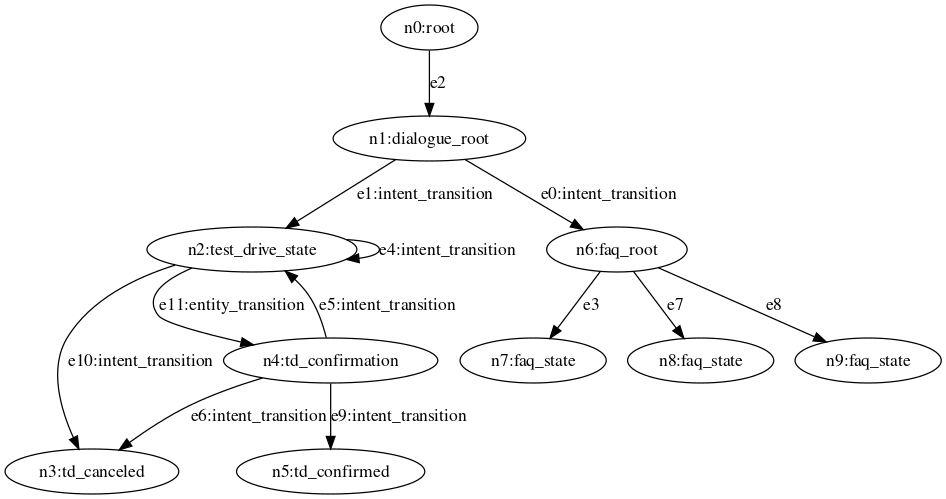
\includegraphics{images/complete.png}

Here comes the biggest benefit of our unified node architecture -- the
exact same walker logic can be shared to traverse both systems. The only
change we need to make is to change from
\passthrough{\lstinline!dialogue\_state!} to
\passthrough{\lstinline!cai\_state!} to apply the walker logic to a more
generalized set of nodes.

\begin{lstlisting}
walker talk {
    ...
    root {
        take --> node::dialogue_root;
    }
    cai_state {
        if (!question) {
            question = std.input("Question (Ctrl-C to exit)> ");
            here::init_wlk_ctx;
        }
        ...
    }
}
\end{lstlisting}

Update the graph name in the \passthrough{\lstinline!init!} walker as
well.

\begin{lstlisting}
walker init {
    root {
        spawn here ++> graph::tesla_ai;
        spawn here walker::talk;
    }
}
\end{lstlisting}

To compile the program,

\begin{lstlisting}
jaseci > jac build tesla_ai.jac
\end{lstlisting}

As mentioned before, if the compiliation succeedd, a
\passthrough{\lstinline!tesla\_ai.jir!} will be generated.

\begin{quote}
\textbf{Note}

Run into issues at this build step? First check if all the imports are
set up correctly.
\end{quote}

Running a \passthrough{\lstinline!jir!} is just like running a
\passthrough{\lstinline!jac!} file

\begin{lstlisting}
jaseci > jac run tesla_ai.jir
\end{lstlisting}

One last step, since we introduce a new intent
\passthrough{\lstinline!i have a questions!}, we need to update our
classifier model again. This time, use the
\passthrough{\lstinline!clf\_train\_3.json!} example training data.

The model is trained? Great! Now run the jir and try questions like ``I
have some telsa related questions'' then following with FAQ questioins!

Congratulations! You have created a single conversational AI system that
is capable of answering FAQs and perform complex multi-step actions.

\hypertarget{bring-your-application-to-production}{%
\section{Bring Your Application to
Production}\label{bring-your-application-to-production}}

Typing in questions and getting responses via
\passthrough{\lstinline!jsctl!} in terminal is a quick and easy way of
interactively test and use your program. But the ultimate goal of
building any products is to eventually deploying it to production and
having it serve real users via standard interface such as RESTful API
endpoints. In this section, we will cover a number of items related to
bringing your jac program to production.

\hypertarget{introducing-yield}{%
\subsection{\texorpdfstring{Introducing
\texttt{yield}}{Introducing yield}}\label{introducing-yield}}

\passthrough{\lstinline!yield!} is a jac keyword that suspend the walker
and return a response, which then can be resumed at a later time with
the walker context retained. Walker context includes its
\passthrough{\lstinline!has!} variables and its node traversal plan
(i.e., any nodes that have been queued by previously executed
\passthrough{\lstinline!take!} statements). This context retention is
done on a per-user basis. \passthrough{\lstinline!yield!} is a great way
to maintaining user-specific context and history in between walker
calls. To learn more about \passthrough{\lstinline!yield,!} refer to the
relevant sections of the Jaseci Bible.

In the case of our conversational AI system, it is essential for our
walker to remember the context information gained from previous
interactions with the same user. So let's update our walker with
\passthrough{\lstinline!yield.!}

\begin{lstlisting}
walker talk {
    has question, interactive = false;
    has wlk_ctx = {
        "intent": null,
        "entities": {},
        "prev_state": null,
        "next_state": null,
        "respond": false
    };
    has response;
    root {
        take --> node::dialogue_root;
    }
    cai_state {
        if (!question and interactive) {
            question = std.input("Question (Ctrl-C to exit)> ");
            here::init_wlk_ctx;
        } elif (!question and !interactive){
            std.err("ERROR: question is required for non-interactive mode");
            disengage;
        }
        here::nlu;
        here::process;
        if (visitor.wlk_ctx["respond"]) {
            here::nlg;
            if (interactive): std.out(response);
            else {
                yield report response;
                here::init_wlk_ctx;
            }
            question = null;
            take here;
        } else {
            take visitor.wlk_ctx["next_state"] else: take here;
        }
    }
}
\end{lstlisting}

Two new syntax here: * \passthrough{\lstinline!report!} returns variable
from walker to its caller. When calling a walker via its REST API, the
content of the API response payload will be what is reported. *
\passthrough{\lstinline!yield report!} is a shorthand for yielding and
reporting at the same time. This is equivalane to
\passthrough{\lstinline!yield; report response;!}.

\hypertarget{introduce-sentinel}{%
\subsection{\texorpdfstring{Introduce
\texttt{sentinel}}{Introduce sentinel}}\label{introduce-sentinel}}

\passthrough{\lstinline!sentinel!} is the overseer of walkers, nodes and
edges. It is the abstraction Jaseci uses to encapsulate compiled walkers
and architype nodes and edges. The key operation with respesct to
\passthrough{\lstinline!sentinel!} is ``register'' a sentinel. You can
think of registering a \passthrough{\lstinline!sentinel!} as a compiling
your jac program. The walkers of a given sentinel can then be invoked
and run on arbitrary nodes of any graph.

Let's register our jac program

\begin{lstlisting}[language=bash]
jaseci > sentinel register tesla_ai.jir -set_active true -mode ir
\end{lstlisting}

Three things are happening here: * First, we registered the
\passthrough{\lstinline!jir!} we compiled earlier to new sentinel. This
means this new sentinel now has access to all of our walkers, nodes and
edges. \passthrough{\lstinline!-mode ir!} option speciifes a
\passthrough{\lstinline!jir!} program is registered instead of a
\passthrough{\lstinline!jac!} program. * Second, with
\passthrough{\lstinline!-set\_active true!} we set this new sentinel to
be the active sentinel. In other words, this sentinel is the default one
to be used when requests hit the Jac APIs, if no specific sentinels are
specified. * Third, \passthrough{\lstinline!sentinel register!} has
automatically creates a new \passthrough{\lstinline!graph!} (if no
currently active graph) and run the \passthrough{\lstinline!init!}
walker on that graph. This behavior can be customized with the options
\passthrough{\lstinline!-auto\_run!} and
\passthrough{\lstinline!-auto\_create\_graph!}.

To check your graph

\begin{lstlisting}[language=bash]
jaseci > graph get -mode dot
\end{lstlisting}

This will return the current active graph in DOT format. This is the
same output we get from running \passthrough{\lstinline!jac dot!}
earlier. Use this to check if your graph is successfully created.

Once a sentinel is registered, you can update its jac program with

\begin{lstlisting}[language=bash]
jaseci > sentinel set -snt SENTINEL_ID -mode ir tesla_ai.jir
\end{lstlisting}

To get the sentinel ID, you can run one of the two following commands

\begin{lstlisting}[language=bash]
jaseci > sentinel get
\end{lstlisting}

or

\begin{lstlisting}[language=bash]
jaseci > sentinel list
\end{lstlisting}

\passthrough{\lstinline!sentinel get!} returns the information about the
current active sentinel, while \passthrough{\lstinline!sentinel list!}
returns all available sentinels for the user. The output will look
something like this

\begin{lstlisting}
{
  "version": null,
  "name": "main.jir",
  "kind": "generic",
  "jid": "urn:uuid:817b4ff4-e6b7-4296-b383-55515e1e8b4a",
  "j_timestamp": "2022-08-04T20:23:16.952641",
  "j_type": "sentinel"
}
\end{lstlisting}

The \passthrough{\lstinline!jid!} field is the ID for the sentinel.
(\passthrough{\lstinline!jid!} stands for jaseci ID).

With a sentinel and graph, we can now run walker with

\begin{lstlisting}[language=bash]
jaseci > walker run talk -ctx {\"question\": \"I want to schedule a test drive\"}
\end{lstlisting}

And with \passthrough{\lstinline!yield!}, the next walker run will pick
up where it leaves off and retain its variable states and nodes
traversal plan.

\hypertarget{tests}{%
\subsection{Tests}\label{tests}}

Just like any program, a set of automatic tests cases with robust
coverage is essential to the success of the program through development
to production. Jac has built-in tests support and here is how you create
a test case in jac.

\begin{lstlisting}
import {*} with "tesla_ai.jac";

test "testing the Tesla conv AI system"
with graph::tesla_ai by walker::talk(question="Hey I would like to go on a test drive"){
    res = std.get_report();
    assert(res[-1] == "To set you up with a test drive, we will need your name and address.");
}
\end{lstlisting}

Let's break this down. *
\passthrough{\lstinline!test "testing the tesla conv AI system"!} names
the test. * \passthrough{\lstinline!with graph::tesla\_ai!} specify the
graph to be used as the text fixture. *
\passthrough{\lstinline!by walker::talk!} specify the walker to test. It
will be spawned on the anchor node of the graph. *
\passthrough{\lstinline!std.get\_report()!} let you access the report
content of the walker so that you can set up any assertion neccessary
with \passthrough{\lstinline!assert!}.

To run jac tests, save the test case(s) in a file (say
\passthrough{\lstinline!tests.jac!}) and import the neccessary walkers
and graphs. Then run

\begin{lstlisting}[language=bash]
jaseci > jac test tests.jac
\end{lstlisting}

This will execute all the test cases in
\passthrough{\lstinline!tests.jac!} squentially and report success or
any assertion failures.

\hypertarget{running-jaseci-as-a-service}{%
\subsection{Running Jaseci as a
Service}\label{running-jaseci-as-a-service}}

So far, we have been interacting jaseci through
\passthrough{\lstinline!jsctl!}. jaseci can also be run as a service
serving a set of RESTful API endpoints. This is useful in production
settings. To run jaseci as a service, first we need to install the
\passthrough{\lstinline!jaseci\_serv!} package.

\begin{lstlisting}[language=bash]
pip install jaseci_serv
\end{lstlisting}

Then launching a jaseci server is as simple as

\begin{lstlisting}[language=bash]
jsserv makemigrations
jsserv migrate
jsserv runserver 0.0.0.0:3000
\end{lstlisting}

This will launch a Django RESTful API server at localhost and port 3000.
The Jaseci server supports a wide range of API endpoints. All the
\passthrough{\lstinline!jsctl!} commands we have used throughput this
tutorial have an equivalent API endpoint, such as
\passthrough{\lstinline!walker\_run!} and
\passthrough{\lstinline!sentinel\_register!}. As a matter of fact, the
entire development journey in this tutorial can be done completely with
a remote jaseci server instance. You can go to
\passthrough{\lstinline!localhost:3000/docs!} to check out all the
available APIs.

\hypertarget{improve-your-ai-models-with-crowdsource}{%
\section{Improve Your AI Models with
Crowdsource}\label{improve-your-ai-models-with-crowdsource}}

Coming soon!
